%--------------------------------
\chapter{Platform}
%--------------------------------
%TODO add citations
Az Android egy nyílt forráskódú, Linux alapú operációs rendszer, mely először okostelefonokra készült, de mára már eszközök igen széles skáláján megtalálható a karóráktól kezdve a háztartási eszközökön át az autókig. A legtöbbet használt mobil operációs rendszer, piaci részesedése közel 73\%.\cite{ShareStat} 

Népszerűsége pedig nem véletlen; a legolcsóbbtól a legdrágábbig mindegyik szegmensben található Android készülék, így mindenki kiválaszthatja a számára legmegfelelőbbet. Hatalmas szabadságot ad a felhasználó kezébe, lecserélhetünk bármilyen alapértelmezett alkalmazást, sőt, akár az operációs rendszert is.

Ez a változatosság és szabadság fejlesztői szempontból kettős. Egyrészről gyakorlatilag lehetséges bármilyen alkalmazást írni, és a nyílt forráskód miatt bármikor bele lehet nézni a platform kódjába, hogy megértsük a viselkedését, másrészről viszont lehetetlenné teszi, hogy ellenőrizni tudjuk az alkalmazásunk működését minden létező készüléken. 

Az alábbiakban a platform felépítését, sajátosságait fogom ismertetni, majd pedig a fejlesztéshez szükséges környezetet és eszközöket mutatom be. 

\section{Felépítés}

A leírás kiegészítéseként a platform felépítését a \refstruc{fig:AndroidPlatform} szemlélteti.
\begin{figure}[!ht]
	\centering
	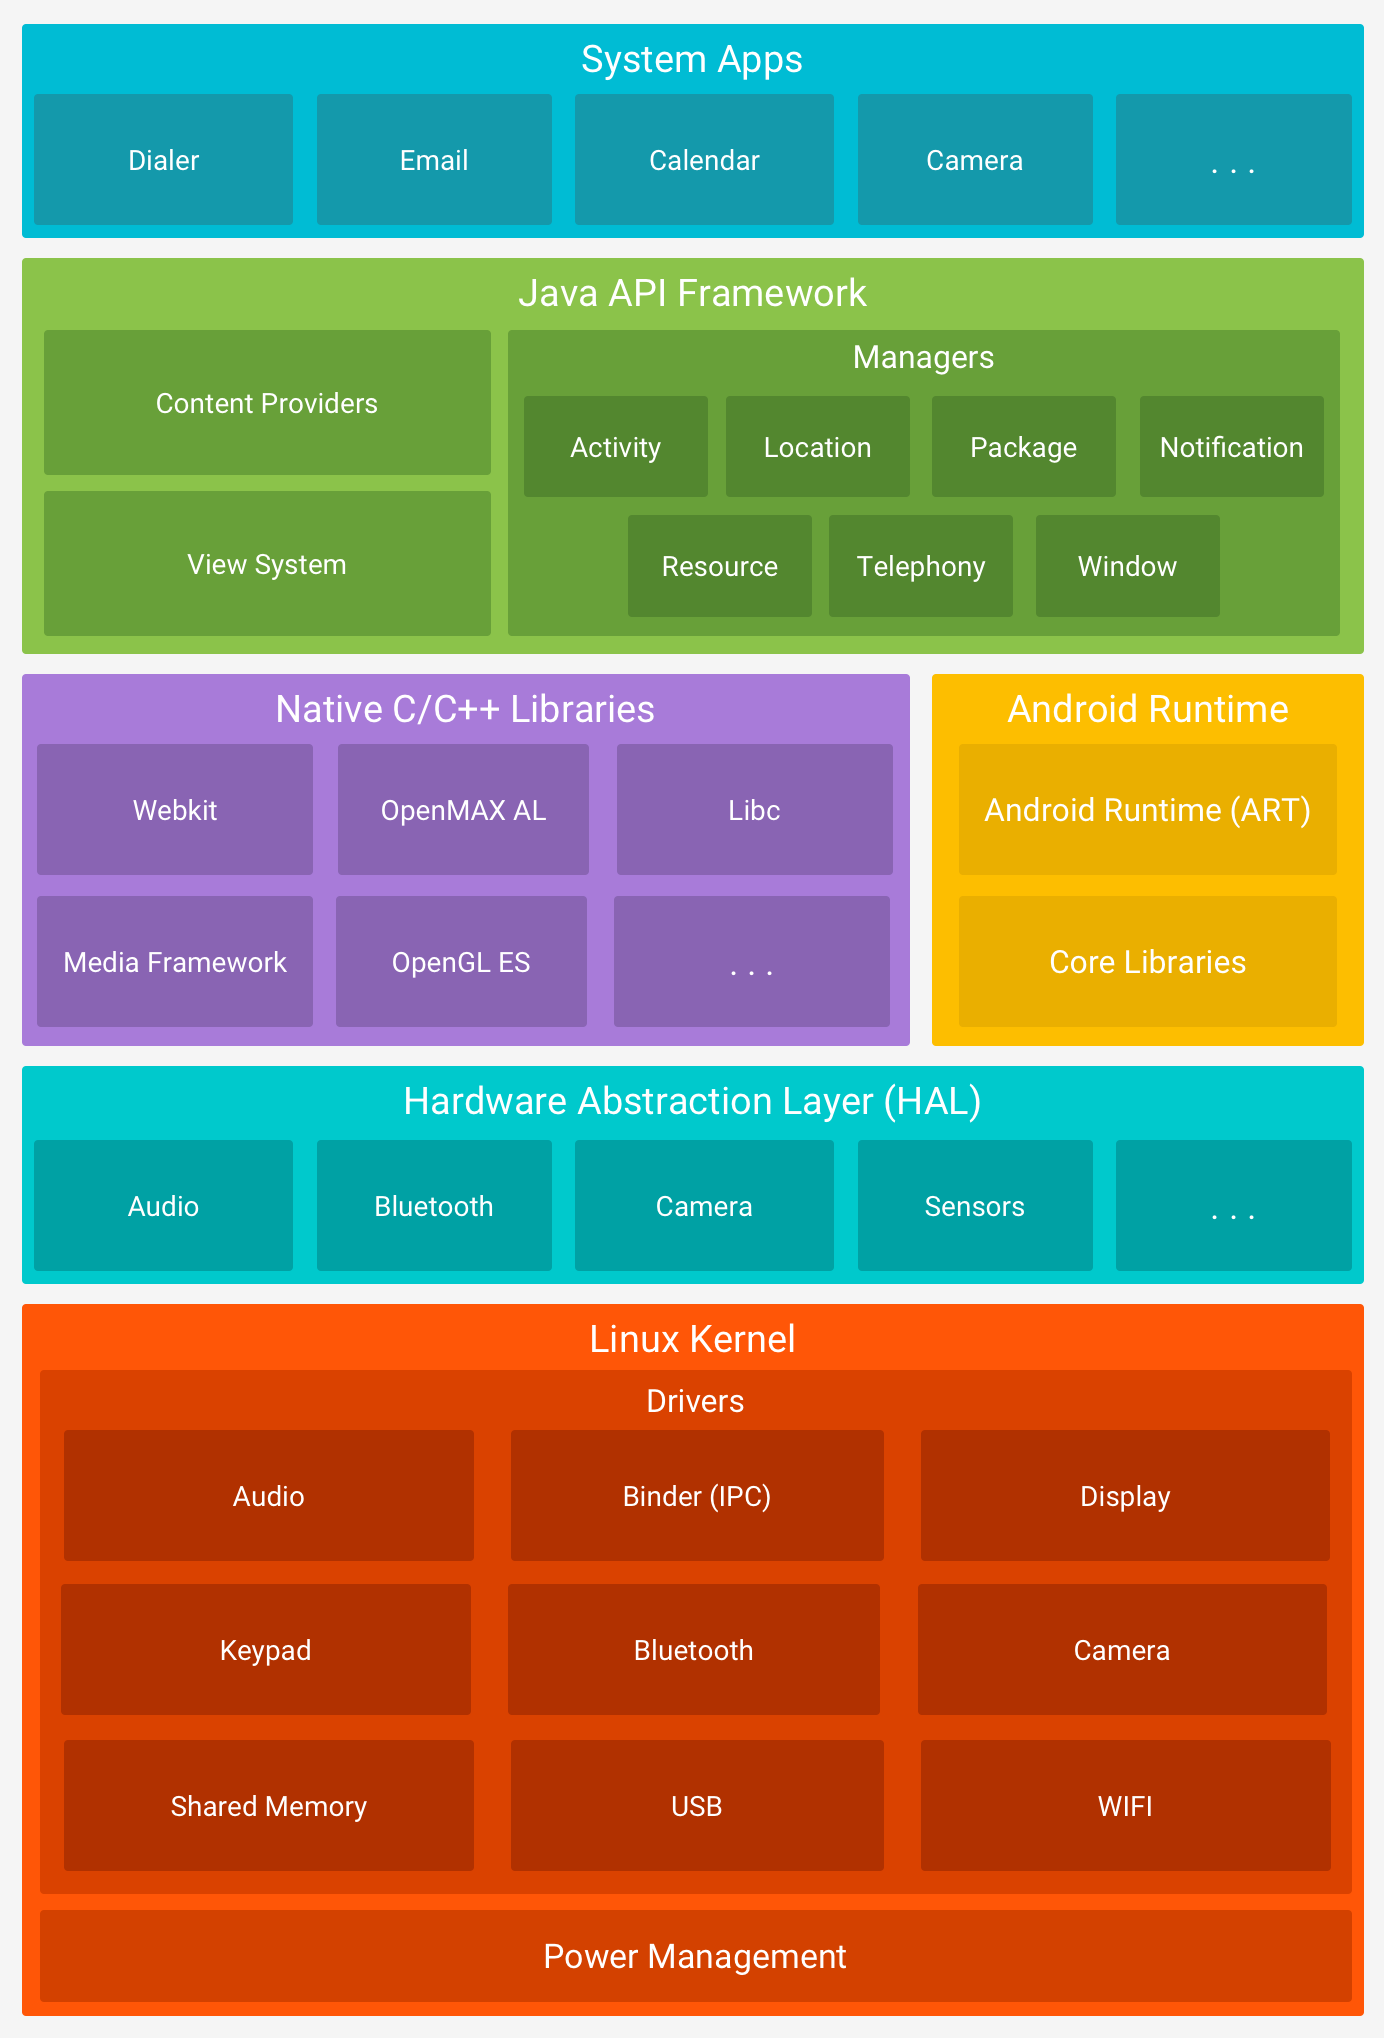
\includegraphics[width=100mm, keepaspectratio]{figures/android-stack_2x.png}
	\caption{Az Android operációs rendszer architektúrája.}
	\label{fig:AndroidPlatform}
\end{figure}

\subsection{Linux kernel}
Az operációs rendszer alapját a Linux kernel képezi, ezáltal ki tudja használni az évek során elért stabilitást és biztonságot, illetve lehetővé teszi a készülékgyártóknak, hogy egy már jól ismert technológiával dolgozzanak az illesztőprogramok fejlesztése során. Feladatai közé tartozik a memóriakezelés, a folyamatok ütemezése és a teljesítménykezelés. Ez utóbbi kiemelt fontosságú, hiszen a mobil eszközök akkumulátora véges, így a lehető legalacsonyabb fogyasztásra kell törekedni. \cite{MobWeb}

\subsection{Hardver absztrakciós réteg}
Közvetlenül a kernel felett található a hardver absztrakciós réteg - hardware abstraction layer, röviden HAL -, mely a készülék hardveres adottságait (pl.: kamera, szenzorok) ajánlja ki a felette található Java API keretrendszernek. Több modulból áll, melyek egy-egy specifikus hardverkomponens interfészt valósítanak meg, és a rendszer dinamikusan tölti be ezeket amikor az API hozzá akar férni valamelyikhez. \cite{PlatformGuide}

\subsection{Android Runtime}
A következő komponens az Android Runtime, röviden ART. Ez egy virtuális gép, melyből mindegyik alkalmazás rendelkezik egy saját példánnyal, így egymástól és az operációs rendszertől izoláltan futhatnak. Mind az ART, mind az elődje, a Dalvik Virtual Machine specifikusan Androidra készültek. Az elődjéhez képest az Android Runtime rendelkezik plusz funkciókkal, ilyen többek között a telepítésidejű fordítás, az optimalizált szemétgyűjtés vagy a jobb hibakeresési támogatás. \cite{PlatformGuide}

\subsection{Natív C/C++ könyvtárak}
Ahogy azt a \refstruc{fig:AndroidPlatform} mutatja, natív C/C++ könyvtárak is helyet kaptak a rendszerben. Ezek a kernelen futnak, és sok rendszerkomponensnek szüksége van rájuk. A platform biztosít Java API-t néhányhoz, így például hozzáférhetünk az OpenGL grafikai könyvtárhoz natív kódból. \cite{PlatformGuide}

\subsection{Java API keretrendszer}
A fejlesztők számára a legfontosabb elem a Java API keretrendszer. Ez tartalmazza az operációs rendszer minden funkcióját, a moduláris, könnyedén újrahasznosítható építőelemeket, melyek felhasználásával a fejlesztők alkalmazásaikat elkészíthetik. Többek között magában foglalja az alábbiakat:
\begin{itemize}
	\item \emph{View System:} Felhasználói felületek létrehozásában van segítségünkre, kiterjedt és még tovább bővíthető elemkészlettel (pl.: listák, szövegmezők, gombok). 
	\item \emph{Resource Manager:} Hozzáférést biztosít a fejlesztőnek minden erőforrásfájlhoz. Ezek tipikusan XML-fájlok, melyek leírják a projektben használatos lokalizált szövegeket, vektorgrafikus ábrákat és a fentebb is említett felhasználói felületeket.
	\item \emph{Activity Manager:} Az Android alkalmazások alapkövei az Activityk, melyeknek meghatározott életciklus-szakaszai vannak a létrehozástól a megszűnésig. Ezt az életciklust kezeli az Activity Manager, illetve egy közös navigációs backstacket biztosít, mely tárolja, hogy az alkalmazásban milyen képernyőket látogattunk meg a használat folyamán. \cite{PlatformGuide}
\end{itemize}

\subsection{Rendszeralkalmazások}
A rendszer beépített alkalmazásokkal érkezik a leggyakoribb feladatok elvégzésére. Ilyen például az SMS-küldés, internet böngészés, telefonálás, naptár és így tovább. Ezek, ahogy a fenti bevezetőben is említettem, néhány kivételével teljesen lecserélhetők felhasználó által letöltött alkalmazásokra. 

Mindez nem csak a felhasználó számára lényeges - a fejlesztő is fel tudja használni. Például, ha a fejlesztő szeretne telefonhívást indítani a saját alkalmazásából, akkor nem kell ezt a funkcionalitást implementálnia, elég csak meghívnia a készüléken elérhető alapértelmezett alkalmazást, ami majd elvégzi ezt. \cite{PlatformGuide}

\section{Fejlesztői környezet}

Az Android fejlesztés hivatalos eszköze az Android Studio, mely egy IntelliJ IDEA alapú integrált fejlesztési környezet, röviden IDE.\cite{AndroidStudio} Rengeteg funkcióval rendelkezik, így most csak a fontosabbakat fogom érinteni. 

\subsection{Funkciók}
\begin{itemize}
	\item \emph{Build eszközök:} Rugalmas, Gradle-alapú build rendszert használ, így a projektbeállításokat és a külső könyvtárakat elég csak az erre kijelölt \emph{.gradle} kiterjesztésű fájlokba felvenni, a többit elvégzi helyettünk.
	\item \emph{Egységes környezet:} Nem kell külön program más eszközökre való fejlesztéshez, akár telefonra, táblagépre vagy okosórára szeretnénk alkalmazást írni, mindet megtehetjük a Studioból. 
	\item \emph{Emulator:} Fejlesztésnél rendkívül praktikus, hogyha nem kell minden alkalommal fizikai készüléket keresni, ha futtatni szeretnénk a programunkat. Erre szolgál az emulátor, amivel virtuális készülékeken tesztelhetünk. Ez egy teljes operációs rendszert tár elénk, így nem csak az alkalmazásunkat tudjuk rajta megnézni, hanem a rendszeralkalmazások is mind elérhetők. Hívásindítást és -fogadást, SMS-eket, konfigurációváltozást vagy akár helyadat-változást is tudunk vele emulálni. Egyszerre több emulátorunk is lehet, ezeket az AVD Managerben tudjuk kezelni. Új létrehozásánál kiválaszthatjuk, hogy milyen készülékmodellt szeretnénk, melyik Android verzióval, és egyéb hardverbeállításokat is megadhatunk, például, hogy mennyi memóriát szeretnénk a készüléknek. 
	\item \emph{Verziókezelés:} Az IDE több verziókezelő rendszert is beépítetten támogat, így egy kényelmes felületen intézhetjük a változtatások követését. 
	\item \emph{Kódelemzési funkciók:} Ezek azok, amik igazán kényelmessé teszik számomra az Android Studio használatát. Folyamatos segítséget nyújt a kódírásban, a kódkiegészítés jelentősen meggyorsítja a haladást. Jelzi, ha bármi elavult, így nem utólag kell megváltoztatni a kódot. Ami viszont számomra a leghasznosabb funkció, az a nem használt kódrészletek jelzése. Mivel az IDE kiszürkíti azokat a változókat és függvényeket, amik egyszer sincsenek meghívva, így könnyű karbantartani, hogy ne maradjon a kódbázisban felesleges sor.
\end{itemize}

\subsection{Projektstruktúra}
Minden projekt egy vagy több modulból áll, és mindent tartalmaz a forráskódtól kezdve a tesztkódon át a build konfigurációkig. A modulok segítségével különálló funkcionalitási egységekre bontható az alkalmazás, melyeket egymástól függetlenül lehet buildelni, tesztelni és debugolni. \cite{ProjectStructure}
Célszerű modulokat használni, ha például különböző eszköztípusokra szeretnénk fejleszteni, hiszen így az egymástól független részeket elkülöníthetjük, de a közös kódot meg tudjuk osztani köztük. 

A fejlesztőkörnyezetet megnyitva a projektfájlok megjelenítése alapértelmezetten eltér a fájlrendszerbeli hierarchiától. Ezt Android nézetnek hívja az IDE, és úgy lett kifejlesztve, hogy a lehető legkényelmesebb legyen a fejlesztők számára. Itt alapvetően három csoportra szedve találhatók meg a forrásfájlok. 

Az első a \emph{manifests}, melyben az \emph{AndroidManifest.xml} fájl található. Ez fontos adatokat tartalmaz az alkalmazásról, melyekre szüksége van a build eszközöknek, az operációs rendszernek, és a Google Play-nek is. Fel kell sorolni benne többek között az összes komponensét, a futás során szükséges engedélyeket (pl.: fájlrendszer-hozzáférés, kamera), illetve a működéshez elengedhetetlen szoftveres és hardveres funkciókat. Utóbbit ellenőrzi is a Play Store, és csak olyan készülékekre engedi feltelepíteni az alkalmazást, melyek ennek megfelelnek. \cite{Manifest}

A következő csoport \emph{java} névre hallgat, és ebben található a projekt összes forráskódja. A nevével ellentétben ma már legtöbbször Kotlin kódot tartalmaz, mivel egy-két éve már ez az Android fejlesztés hivatalos nyelve, de az elnevezés megmaradt azokból az időkből, amikor még mindenki Java-t használt. 

Az utolsó csoport pedig a \emph{res}, melyben az erőforrásfájlok találhatók. Ezek általában XML fájlok, és az alkalmazásban felhasznált layoutokat, animációkat, stringeket írják le, de ide kerülnek például a képi erőforrások is. 